\documentclass[titlepage]{article}
\usepackage{graphicx} % Required for inserting images
\usepackage{float} % For tables and figures
\usepackage{amsmath} % For any special symbols
\usepackage{geometry} % Margins
\usepackage{lineno} % Line numbers
\usepackage{parskip} % Paragraph formatting
\usepackage{mathptmx} % Roman font
\usepackage[T1]{fontenc} % Roman font
\usepackage{helvet} % Helvetica (doesn't seem to do anything)
\usepackage[dvipsnames]{xcolor} % Coloring text
\usepackage{titlesec} % Formatting section and subsection headers
\usepackage{url} % Works Cited
\usepackage{hyperref} % Makes works cited cleaner
\usepackage{listings}
\usepackage{verbatim}
\usepackage{wrapfig}
\usepackage{pgfplots}
\pgfplotsset{compat=1.18}
\usepackage[labelsep=space]{caption}
\usepackage{mathtools}
\usepackage[
backend=biber,
style=ieee
]{biblatex}
\addbibresource{sunprojectreference.bib}

\definecolor{codegreen}{rgb}{0,0.6,0}
\definecolor{codegray}{rgb}{0.5,0.5,0.5}
\definecolor{codepurple}{rgb}{0.58,0,0.82}
\definecolor{backcolour}{rgb}{0.95,0.95,0.92}

\lstdefinestyle{mystyle}{
    backgroundcolor=\color{backcolour},   
    commentstyle=\color{codegreen},
    keywordstyle=\color{magenta},
    numberstyle=\tiny\color{codegray},
    stringstyle=\color{codepurple},
    basicstyle=\ttfamily\footnotesize,
    breakatwhitespace=false,         
    breaklines=true,                 
    captionpos=b,                    
    keepspaces=true,                 
    numbers=left,                    
    numbersep=5pt,                  
    showspaces=false,                
    showstringspaces=false,
    showtabs=false,                  
    tabsize=2
}

\lstset{style=mystyle}

\geometry{
    a4paper,
    top=1.3in,
    bottom=1.3in,
    left=1.25in,
    right=1.25in
}

\newcommand{\degree}{$^{\circ}$}

\author{Owen Colburn \\ Math Lab Consultant \\ Michigan Technological University}
\title{Sun Project Overview and Procedure}

\begin{document}
\maketitle

\section*{Overview}
This project explores the usage of real-world data to allow a solar panel to track the sun's movements across the sky. This project relies on no optics, photo sensors, or heated gas to correctly orient the panel, and at least on a small scale represents an efficient way to monitor the sun's movements throughout the day. \par
Real world data about the sun's position is calculated and collected using \textit{Mathematica}, a software not just for mathematics, but also for "neural networks, machine learning, image processing, geometry, data science, visualizations and much more." \cite{mathematica} The data is collected at the start of each day, for every 15 minute interval throughout the day. \par

\begin{wrapfigure}{r}{0.5\linewidth}
    \centering
    \includegraphics[width=0.5\linewidth]{images/image.png}
    \caption{Altitude and Azimuth Visualization \cite{sun_azimuth_image}}
\end{wrapfigure}

Each data point collected is a pair; the angle, or "altitude", and the azimuth of the Sun as seen from Houghton, Michigan. The altitude is defined as the angle of the sun above the horizon, measured from -90\degree to 90\degree. It can generally be said that sunrise occurs when the altitude of the sun goes from negative to positive, and sunset occurs when the altitude goes from positive to negative. The azimuth is defined as the clockwise rotation from North of the Sun. This value ranges from 0\degree to 359\degree. \par

This pair is then nicely formatted into a table and exported to a spreadsheet. Every 15 minutes, this spreadsheet is parsed and the azimuth for that time is retrieved. The azimuth value is then written to a Liquid Crystal Display (LCD) screen, and a Servo motor rotates to align itself with the sun. \par

\normalsize
This project is packaged into a 3D printed box that contains all peripherals and wires within it. This box displays information about software to run the project, and is inscribed with the hardware pieces to go in each place to aid in construction. \par

The final example project was soldered together using a prototype board, but that process isn't covered here.

\section*{Skills Explored}
This project is a celebration of multiple different knowledge bases. Each must work together with the others in order to be succesful. These knowledge bases can be generalized into seven major categories: Raspberry Pi, Mathematica, Python, peripheral devices, circuitry, 3D design and printing, and troubleshooting. \par
\subsection*{The Terminal}
Throughout this report, it is referenced many times to ``run the following command." Commands are run in the terminal, which can be accessed by clicking the icon located in the top left of the Raspberry Pi Desktop. The terminal is used to run commands or open files without the need for a graphical interface. All commands presented should be typed exactly as they appear in order to work properly. \par
\subsection*{Raspberry Pi}
The main hub of this project is the Raspberry Pi, described by its manufacturer as "[the] big computer that fits in your hand."\cite{raspberry_pi} These are low cost computers that operate using Linux. A Raspberry Pi can be used to do anything that a regular laptop or desktop computer is capable of and then some. This is mainly achieved through the Raspberry Pi's 40 general purpose input/output (GPIO) pins, pictured below. \par

\begin{figure}[H]
    \centering
    \includegraphics[width=0.5\linewidth]{images/Raspberry-Pi-GPIO-Header-with-Photo.png}
    \caption{GPIO Header for Raspberry Pi}
\end{figure}

The Raspberry Pi also includes support for USB devices, multiple HDMI displays, and a wired internet connection via ethernet. All this to say, the Raspberry Pi is a powerful, low cost computer that was perfect for this project. \par
\subsubsection*{Cron Job}
One specific feature of the Linux operating system that was leveraged for the most success was the cron job. "A cron job is a Linux command used for scheduling tasks to be executed sometime in the future."\cite{cron_job} Scheduling a cron job only requires a couple of commands and the syntax for the job itself is rather simple. Setting up the specific job for this project will be covered later, but to view any existing jobs, run the following command:
\begin{lstlisting}[language=bash]
crontab -l
\end{lstlisting}
This command will open up a configuration file that details more closely what a cron job is, the syntax for setting up a job, and will list any currently existing cron jobs that have been set up by the user. \par
Utilizing a cron job is extremely helpful for the optimized usage of computational resources. Being able to automatically run at a set interval removes the need for a long delay in software, which would eat up valuable computational power while the project sits in idle. This change could allow for more projects to be run off the same Raspberry Pi at the same time. 
\subsubsection*{Pin Factory}
One of the main benefits of using a Raspberry Pi over a standard laptop or desktop computer is the ability to utilize the 40 GPIO pins. There is however a significant challenge between the software instruction and the hardware interpretation to use a pin. This is where the pin factory comes in. \par
According to the GPIO Zero library documentation, ``When you construct a device, you pass in a pin specification. This is passed to a pin Factory which turns it into a Pin implementation."\cite{pin_factory} The pin factory is what translates between a software instruction, and a manifested real-life signal. \par
The default pin factory on a Raspberry Pi with the RPiGPIO library is the RPiGPIOFactory. Some devices, like the Servo used in this project, interface better with other pin factories. The PiGPIOFactory used in this project comes from the GPIO Zero library. 
\subsection*{Mathematica}
\textit{Mathematica} is a powerful software tool that has applications in many areas of STEM. While its main usage is in mathematics, \textit{Mathematica} also contains the Wolfram Knowledgebase, a vast knowledge base that allows for search and collection of "up-to-the-minute real-world data across thousands of domains."\cite{mathematica} The Wolfram Knowledgebase is what curates the data for the sun's daily positions. \par
One other benefit of \textit{Mathematica} is its large number of built in functions. In this project, \textit{Mathematica} functions are used to retreive the sun's data, format the data into two columns, and export the data into a spreadsheet. 
\subsection*{Python}
The main software used in this project is Python. Python is a free, open-source software language that is very beginner friendly. The Python syntax rules are too broad to be shared here, so it's necessary to have a fundamental understanding of Python before beginning this project. \par
\subsubsection*{Libraries}
While powerful in its base package, Python developers have added ``libraries" to add easier access to functionality. Some of the libraries are used to allow for connection with peripheral devices like a Servo or LCD, and others allow the program to be told to wait for a set period of time. Using libraries like these ensure that the programmer doesn't have to write what could end up being very complicated code to acheive a simple task. \par
Libraries are included in a project using Python's import statement. In some instances, the library itself can be too clunky to manage and access. In those cases, where the programmer only requires a few modules from that library, those can be accesed using the keyword ``from", like so:
\begin{lstlisting}[language=python]
from LIBRARY import MODULE
\end{lstlisting}
Using the sleep module from the time library as an example: 
\begin{lstlisting}[language=python]
from time import sleep
\end{lstlisting}
Part of writing good code is writing clean-looking code, and using the ``from" keyword when appropriate is a good way to clean up a codebase.
\subsection*{Peripheral Devices}
The large functionality of the Raspberry Pi mainly comes from its ability to connect to peripheral, or outside, devices and then control them with software. These devices range from ultrasonic sensors, to buzzers, to seven-segment displays and so much more. 
\subsubsection*{Servo}

\begin{wrapfigure}{r}{0.5\linewidth}
    \centering
    \includegraphics[width=0.5\linewidth]{images/servoInPrint.jpeg}
    \caption{Servo Motor in 3D Print}
\end{wrapfigure}

One of the devices used in this project is a SMRAZA SG90 9g Servo motor. These motors have 180\degree rotation and are controlled through a process known as PWM or pulse-width modulation. ``Pulse-width modulation is a digital technique to control a signal by repeatedly toggling a signal between a HIGH and a LOW state in a consistent pattern." \cite{pulse_width_modulation} This toggling changes the average power being delivered to the servo, and the incoming signal communicates with the driver inside the servo to rotate the motor to the desired angle. \par

One of the unique challenges with using a small servo like the one in this project, is that the servo is not a continous rotation motor. This means that there are limits to how much it can rotate [Fig. 4]. 

\begin{figure}[H]
    \centering
    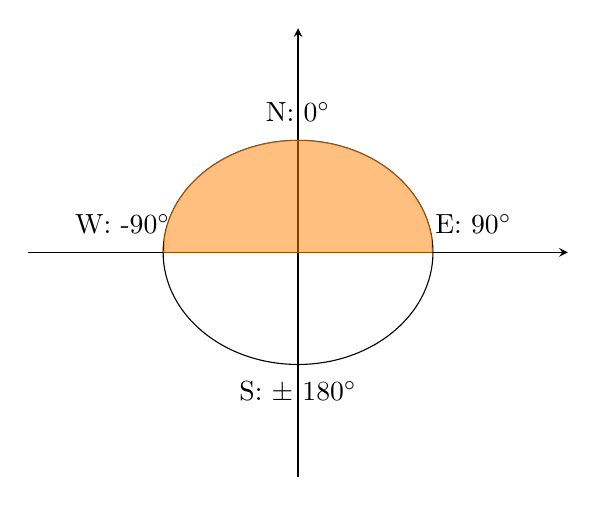
\begin{tikzpicture}
        \begin{axis}[
            ticks = none,
            axis lines = center,
            xmin = -2, xmax = 2,
            ymin = -2, ymax = 2]
            \draw (axis cs: 0,0) circle [radius=1];
            \addplot+ [fill, color=orange, opacity=0.5, samples=500, mark=none] {(1-x^2)^(0.5)} \closedcycle;
            \node at (axis cs: 1.3,0.25) {E: 90\degree};
            \node at (axis cs: 0,1.25) {N: 0\degree};
            \node at (axis cs: -1.3,0.25) {W: -90\degree};
            \node at (axis cs: 0,-1.25) {S: $\pm$ 180\degree};
        \end{axis}
    \end{tikzpicture}
    \caption{Servo Rotation Angles in Relation to Cardinal Directions}
\end{figure}
The motor only has a range of -90\degree to 90\degree. When dealing with sun angles greater than 90\degree, the software will have to adjust the value being sent to the servo. To do this, its necessary to recall the geometry of the problem. To acheive the maximum rotation of 90\degree, the servo must be passed a value of -1. To acheive the minimum rotation, the value must be 1. This could be expressed mathematically using these formulas: 
\begin{equation*}
    \begin{split}
        \textrm{deg\_to\_ms}(90) & = -1 \\
        \textrm{deg\_to\_ms}(-90) & = 1
    \end{split}
\end{equation*}
The operation to acheive this is fairly simple, and is just standard division. This would give a ``deg\_to\_ms(deg)" function as 
\begin{equation}
    \textrm{deg\_to\_ms(deg)} = \frac{-\textrm{deg}}{90}
\end{equation}
This is a correct function, but it won't work for degree values greater than 90. Knowing that two angles 180\degree apart are opposite angles, any angle greater than 90 can simply have 180\degree subtracted off, and the servo rotated to the position given by $\frac{-(\textrm{deg} - 180)}{90}$. In the code, that looks like this, using a ternary statement.
\begin{lstlisting}[language=Python]
def deg_to_ms(deg, servo):
    servo_value = -(deg-180)/90 if deg > 90 else -deg/90 \end{lstlisting}

Since the servo has two arms pointing 180\degree away from each other, the angle still appears to be correct.

 
\subsubsection*{LCD}
Having the servo pointing in two different directions can lead to ambiguity of what angle is actually being represented. To remove any potential ambiguity, the angle on the servo is being displayed using a Liquid Crystal Display, [Fig. 5]. This screen is connected via the I$^2$C (pronounced "I-squared-C") protocol to the Raspberry Pi. This protocol greatly simplifies the wiring required for the LCD to operate, requiring just two input signals (other than power and ground) rather than a standard 14. \par
\begin{figure}[H]
    \centering
    \includegraphics[width=0.5\linewidth]{images/LCDInPrint.jpeg}
    \caption{LCD Displaying Azimuth Value}
\end{figure}
The I$^2$C protocol uses the SDA and SCL GPIO outputs from the Pi to operate. SDA is a ``Serial Data" pin and SCL is the ``Serial Clock" pin. In the case of this project, SDA is used to transmit the message to be displayed on the LCD, and SCL is used to synchronize the transmission between the display and the Pi. \par
While the wiring of the LCD to the Pi is rather simple, actually sending instructions to the LCD is rather difficult. In order to communicate with the LCD, a seperate driver file is necessary. This file introduces easy functions for writing to the LCD, and works over an I$^2$C connection. Downloading and importing this file will be discussed later. 
\subsection*{Circuitry}
The multiple devices used in this project must be physically connected in some manner. This is acheived by creating a circuit. Each device is called a ``circuit component", and is connected to the circuit via wires. Wires used in this project are either ``male-to-female" or ``male-to-male". A male to female wire has a protruding point on one end and a socket on the other. A male to male wire has two protruding points, one on each end. 
\subsubsection*{Breadboard Connections}
To connect each component to each other, a breadboard is used. The breadboard is one of the most fundamental pieces in electronics prototyping and small-scale electronics devices. The breadboard allows for connections to be made between the Raspberry Pi and peripheral devices with ease. Two long sides of the breadboard are adorned with a red and blue line; marked with a red + and a blue -. The red line is a positive power line, and the blue line is a ground line. These lines are connected all the way down the length of the breadboard. \par
In the middle of the board, there are 30 (or more, depending on the size of the breadboard) rows of five columns. Each row is connected to each other, on that side of the breadboard. In each row, the first five columns are connected with each other, and the second five columns are connected with each other. Columns in the same row, but on different sides of the line running down the middle of the board, are NOT naturally connected. \par
More advanced students could find it a worthy challenge to design, print, and use a PCB (printed circuit board) or prototype-board instead of a breadboard, especially if this project is intended to be more permanent or the student has an interest in learning PCB design, manufacturing, and soldering. The necessary steps to design, manufacture, and solder the PCB won't be covered here. \par
\subsection*{3D Design and Printing}
While the project can live on its own, a 3D printed housing for the project can elevate the overall look and quality of the finished product. Designing the housing can be done using any CAD software, and printed using a 3D printer. The example project was designed in TinkerCAD, and printed using a Flashforge printer. \par
When designing the housing, there are a few things to keep in mind. First of all, the housing must fit the Servo, LCD, and breadboard. The Servo and LCD should be displayed in the front, and the breadboard can be tucked away underneath. Make sure that the overall footprint of the design is large enough to fit all components. Secondly, its important to make sure that there is enough room for the wires to pass through the middle of the print. If the wires can't pass through, the circuit can't be wired, and won't operate when in the housing. Make sure that there is enough room to manipulate the wires. There shouldn't be any sharp angles for wires to pass around as this could damage the wires in the long run if held in that position. \par
Finally, make sure the holes for the components are big enough to fit, but have some tolerance on the measurements. These components are fragile, and shouldn't be shoved into a space they can barely fit. Add a few millimeters to the dimensions of the components in order to ensure a comfortable, snug, fit. \par
Once the part is designed, it can be sliced and printed using a 3D printer and other relavent software. 
\subsection*{Troubleshooting}
In engineering, oftentimes the individual components can work well on their own, but combining them can lead to many issues. Here are some of the common issues that may arise during the making of this project, and some tips on how to fix them. \par
\begin{enumerate}
    \item Components not turning on, or working properly \par
    For components not turning on, check the circuit construction and make sure that each wire is connected correctly and securely into the breadboard. If the components turn on but aren't working correctly, either by outputing the wrong value, or not outputing anything at all, check the circuit for bad connections, and check the software for any bugs or undefined behaviour.
    \item LCD not displaying anything \par
    The I2C\_LCD\_driver.py file requires an address for the LCD. To ensure the correct address is listed in the code, follow the steps in ``Setting up the LCD". 
    \item Python \lstinline[language=Python]{FileNotFoundError} \par
    This error arises when Python can't find the file specified to a function through the given path. The provided code includes variables for the \textit{Mathematica} file location and the location of the sun data sheet. These paths need to be updated before the code can work properly. 
    \item Python \lstinline[language=Python]{ModuleNotFoundError} \par
    This error arises when a module being imported by the code can't be found on the device. This error can be caused by many things, but is usually caused by either the module name not being spelled correctly in the code, or the module not being installed on the device. This second issue can be rectified by going back to the terminal, and running:
    \begin{lstlisting}[language=bash]
pip3 install MODULE_NAME \end{lstlisting}
    where \lstinline[language=Python]{MODULE_NAME} is replaced by the module that you want to install. Keep in mind that when running a file via a cron job that any errors in the code will be output to a log file, not the terminal. It may be necessary to use a try-except statement, or print statements to debug any issues when running via a cron job. 
    \item Network Issues and MAC Address Randomization \par
    The Mathematica code is written to not require an internet connection in order to work, but the Raspberry Pi will need an internet connection to know what time it is. On a managed network, like a school or business, the device may need to be registered with the network in order to connect. When registering the device, it may ask for a MAC address. If the Raspberry Pi has NetworkManager installed on it, MAC Address Randomization could be on and the device may not properly sync the time on the next startup. To turn off MAC Address randomization, run the following commands in the terminal:
    \begin{lstlisting}[language=bash]
nano /etc/NetworkManager/NetworkManager.conf    \end{lstlisting}
    This will open the configuration file for the network manager. If this file is empty, then NetworkManager isn't installed and there's nothing you need to do. Simply exit out of the file and delete it. If the file isn't empty, there should be a line that says:
    \begin{lstlisting}[language=bash]
[device]
wifi.scan-rand-mac-address=yes \end{lstlisting}
    Change the \lstinline[language=bash]{yes} to a \lstinline[language=bash]{no}, so the file looks like this
    \begin{lstlisting}[language=bash]
[device]
wifi.scan-rand-mac-address=no \end{lstlisting}
    Reboot the Pi, and check the MAC address by running
    \begin{lstlisting}[language=bash]
ifconfig   \end{lstlisting}
    and looking for the MAC Address after the word \lstinline[language=bash]{ether}. This is the address that should be registered with the network.
\end{enumerate}
\section*{Procedure}
\LARGE{\textbf{Safety Consideration}} \\
\normalsize
\textbf{Never} work on a live circuit. When wiring the circuit together, always make sure that the Raspberry Pi is unplugged, and you are grounded while working on the circuit. You can ground yourself by either wearing an antistatic wristband, or touching large exposed metal parts before touching the circuit to safely discharge any built up charge on your skin. The voltages and currents in such a small project are unlikely to hurt you, but the build up of charge on your skin can destroy the Raspberry Pi if not properly discharged. 
\subsection*{Materials Needed}
\begin{itemize}
    \item Raspberry Pi 5
    \item 9g Servo Motor
    \item 16x2 LCD with I$^2$C backpack
    \item 400pt Breadboard
    \item 12 Male to female wires
    \item 5 Male to male wires
    \item A microSD card to install the Raspberry Pi OS, if not done so already
    \item Keyboard
    \item Mouse
    \item Monitor connected to the Pi via micro-HDMI.
\end{itemize}
\medskip
\begin{enumerate}
    \item Make sure the Raspberry Pi is set up according to the instructions \cite{raspi_setup}. The Raspberry Pi desktop should be visible on the screen, with a mouse and keyboard connected.
\subsection*{Software}
    \item Download the code files for this project from \cite{github} onto a USB drive.
    \item Connect the USB drive to the Raspberry Pi. 
    \item In the folder of the Raspberry Pi with the same name as the user (i.e. ``/home/USER/), create a folder called sunProject. The file path should look like this: ``/home/USER/sunProject.
    \item Transfer the code files from the USB to the new folder.
\subsubsection*{Mathematica}
    \item Mathematica is installed on every Raspberry Pi. It can be accessed by clicking the icon in the top left of the Raspberry Pi, hovering over ``Programming" and clicking on ``Mathematica". 
    \item Once Mathematica is open, click the option to ``Open".
    \item Navigate to the ``sunProject" folder and double-click the ``sunCode-1.nb" file to open it.
    \item To get the current location coordinates of the Raspberry Pi, run FindGeoLocation[]. Update the values in the GeoLocation function to match.
    \item Save the file.
\subsubsection*{Python}
    \item Make sure that the Raspberry Pi has the most up to date version of Python installed by running
    \begin{lstlisting}[language=Python]
sudo apt-get install python3 \end{lstlisting}
    \item In the ``sunProjectMain.py" file, ensure that the ``MATHEMATICA\_FILE\_PATH" and \\ ``SUN\_DATA\_FILE\_PATH" are both correct. They should look like this: 
    \begin{lstlisting}[language=Python]
MATHEMATICA_FILE_PATH = "/home/USER/sunProject/sunCode-1.nb"
SUN_DATA_FILE_PATH = "/home/USER/sunProject/sunData.ods" \end{lstlisting}
\subsubsection*{Setting up the LCD}
    The contents of this section are taken from \cite{lcd_driver_location}
    \item In the terminal, enter
    \begin{lstlisting}[language=bash] 
sudo raspi-config    \end{lstlisting} 
    to access the configuration menu. Arrow down to ``Advanced Settings".
    \item Arrow down to ``I2C Enable/Disable automatic loading"
    \item Choose ``yes", exit the configuration menu, and reboot the Pi.
    \item Back in the terminal, enter
    \begin{lstlisting}[language=bash] 
sudo apt get-install i2c-tools    \end{lstlisting}
    \item Once that's installed, enter
    \begin{lstlisting}[language=bash] 
sudo apt get-install python-smbus    \end{lstlisting}
    \item Reboot the Pi once again.
    \item Connect the LCD to the Raspberry Pi. The SDA signal connects to pin 3, the SCL connects to pin 5, the VCC connects to pin 2, and the GND connects to pin 6. These connections can be made via the breadboard.
    \item With the LCD connected, enter
    \begin{lstlisting}[language=bash] 
i2cdetect -y 1     \end{lstlisting}
    This will bring up a menu showing all the addresses of any connected I$^2$C devices. Make note of the address of the LCD.
    \item In the ``I2C\_LCD\_driver.py" file, change the value of ``ADDRESS" on line 22 to match the address from the previous step. 
\subsubsection*{Setting up the Cron-job}
    \item To view, edit, or add a cron job, open the terminal and enter
    \begin{lstlisting}[language=bash]
crontab -e    \end{lstlisting}
    \item At the end of the file, add
    \begin{lstlisting}
0,15,30,45 * * * * python3 /home/USER/sunProject/sunProjectMain.py \end{lstlisting}
    \item Save and exit the file.
\subsection*{3D Printing (Optional)}
    \item Measure the dimensions of the LCD and Servo motor. 
    \item Using CAD software, design a housing for the project. It should include a space ``set-in" the box for the LCD and the Servo, and channels inside the box for wires to be passed through. Ensure that the spaces for the LCD and Servo are a few millimeters larger than the actual dimensions of the components to allow for a snug fit. 
    \item Export the completed design as a .stl file. 
    \item Import the .stl into a slicing software.
    \item Configure the slice parameters, and slice the .stl. Export the sliced .stl in the preferred file format for your printer (.g, .gcode, .gx) to a USB drive. 
    \item Connect the USB to the printer, and select the sliced .g or .gx file. 
    \item Begin the print. Based on the size of the model and printing parameters, the print could take up to 12 hours.
\subsection*{Assembling}
    \item Ensure that the Raspberry Pi has been \textbf{disconnected from power.} (See the ``Safety Consideration" above).
    \item Connect pins 2 and 6 from the Raspberry Pi onto the red and blue lines on one of the long rails on the breadboard, respectively. Use a red wire for pin 2, and a black wire for pin 6, as is convention.
    \item Connect pins 3, 5, and 11 from the Raspberry Pi onto three different rows in the middle of the breadboard. Use the same color wire for pins 3 and 5. Use a different color for pin 11.  
    \item Use two male to male wires to connect the power rails on opposite sides of the breadboard together. 
    \item Use three male to male wires to connect the wires from pins 3, 5, and 11 to the other side of the breadboard. 
    \item Place the LCD in the desired slot, passing the wires through the channel of the housing. Depending on the length of the wires, they may appear out on the other side. Make note of which wire is the SDA signal, and which one is the SCL signal. 
    \item Place the Servo in the desired slot, passing the wires through the channel in the housing. Depending on the length of the wires, they may appear out on the other side. 
    \item Connect the power and ground of the LCD and Servo to the opposite power rail. 
    \item Connect the SDA signal from the LCD to the output of pin 3.
    \item Connect the SCL signal from the LCD to the output of pin 5.
    \item Connect the signal input of the Servo to the output of pin 11. 
    \item At this point, the Raspberry Pi can be plugged back in. If the wiring has been done correctly, the LCD should light up, and the servo may rotate. 
\subsection*{Testing}
    \item In the terminal of the Pi, enter the following commands to set the time just before midnight. 
    \begin{lstlisting}
sudo systemctl stop systemd-timesyncd.service 
timedatectl set-time "2025-03-31 23:59:30"
timedatectl   \end{lstlisting}
    \item This should now show the local time as ``2025-03-31 23:59:30". 
    \item In 30 seconds, the Raspberry Pi should now think that it's midnight, and will run ``sunProjectMain.py". It should see that since it's midnight, it will need to run the \textit{Mathematica} file, and the LCD should display ``Gathering Data..." 
    \item Once ``Gathering Data" goes away, the LCD should display ``Data collected!" before printing ``Current Azimuth: " with an azimuth value printed beneath it. The Servo should rotate to match this value. 
    \item If the LCD isn't displaying properly, or the Servo doesn't rotate, review the ``Assembling" section to ensure that the connections are correct. If they are, double check the software. 
    \item If everything is working properly, then run 
    \begin{lstlisting}
sudo systemctl start systemd-timesyncd.service  \end{lstlisting}
    This should restart the time synchronization service, and assuming the Pi is connected to the internet, the time should update to the correct local time. \par
    Code snippets for ``Testing" taken from \cite{time_sync}.
\end{enumerate}

\newpage

\section*{Appendix}
\subsection*{Code}
\subsubsection*{Appendix A. I2C\_LCD\_driver.py}
This file was accessed from \cite{lcd_driver_location}, originally posted on \cite{original_lcd_driver_location}, and was updated and further developed by \cite{DenisFromHR}.
\lstinputlisting[language=Python]{Code/I2C\_LCD\_driver.py}
\subsubsection*{Appendix B. sunProjectMain.py}
\lstinputlisting[language=Python]{Code/sunProjectMain.py}
\subsubsection*{Appendix C. sunCode-1.nb}
\lstinputlisting[language=Mathematica]{Code/sunCode-1.nb}
\section*{Acknowledgment}
Beaumont Ujlkay - For all the help with 3D printing \\
The Michigan Technological University Math Lab - for a work space, project components, and 3D printing capabilities. \\
Math Lab Director Dr. Jason Gregersen - for approval, funding, and guidance throughout the project. 

\newpage

\printbibliography

\end{document}

